\documentclass{beamer}

\mode<presentation>

\title{Music Similarity}
\subtitle{Flash Representation}
\author{Ali Bektas \and Paul Kröger}

\usepackage{graphicx}
\graphicspath{{./images/}}
\usepackage{verbatim}

\begin{document}
	\begin{frame}
		\maketitle
	\end{frame}
	\begin{frame}
  		\frametitle{Was wir machen}
  		\begin{itemize}
  			\item Symbolic Melodic Music Similarity 
  			\begin{itemize}
  				\item "symbolisch" heißt : Darstellung von Noten.
  				\item verschiedene Representationsansätze von Melodien 
  			\end{itemize} 
			\item 3 grundlegende Klassen von Algorithmen : diejenigen ,
			\begin{itemize}
				\item die Mathematik einsetzen
				\item die musiktheoretische Ansätze verfolgen
				\item noch was.
			\end{itemize}
			\item und hybride Methoden(\textit{lineare Kombination} von Algorithmen).
  		\end{itemize}
	\end{frame}
	\begin{frame}
  		\frametitle{Wie man es macht}
  		\begin{figure}[h!]
					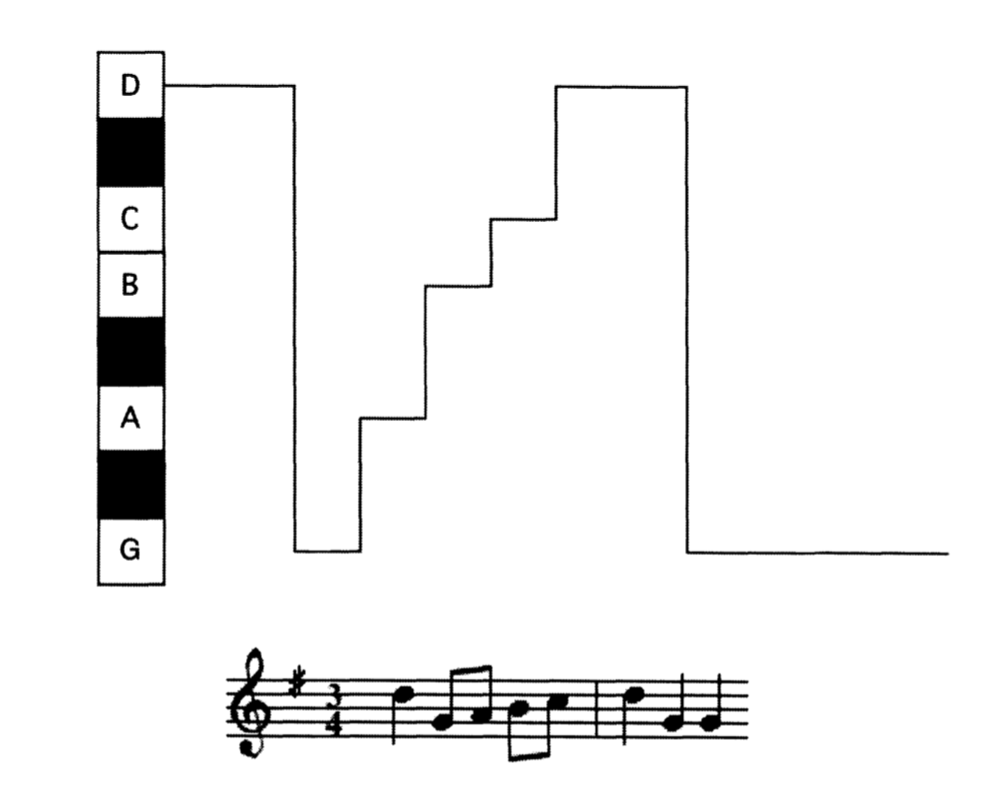
\includegraphics[width=300px,height=100px,keepaspectratio]{abb_1}
		\end{figure}
		\begin{figure}[h!]
					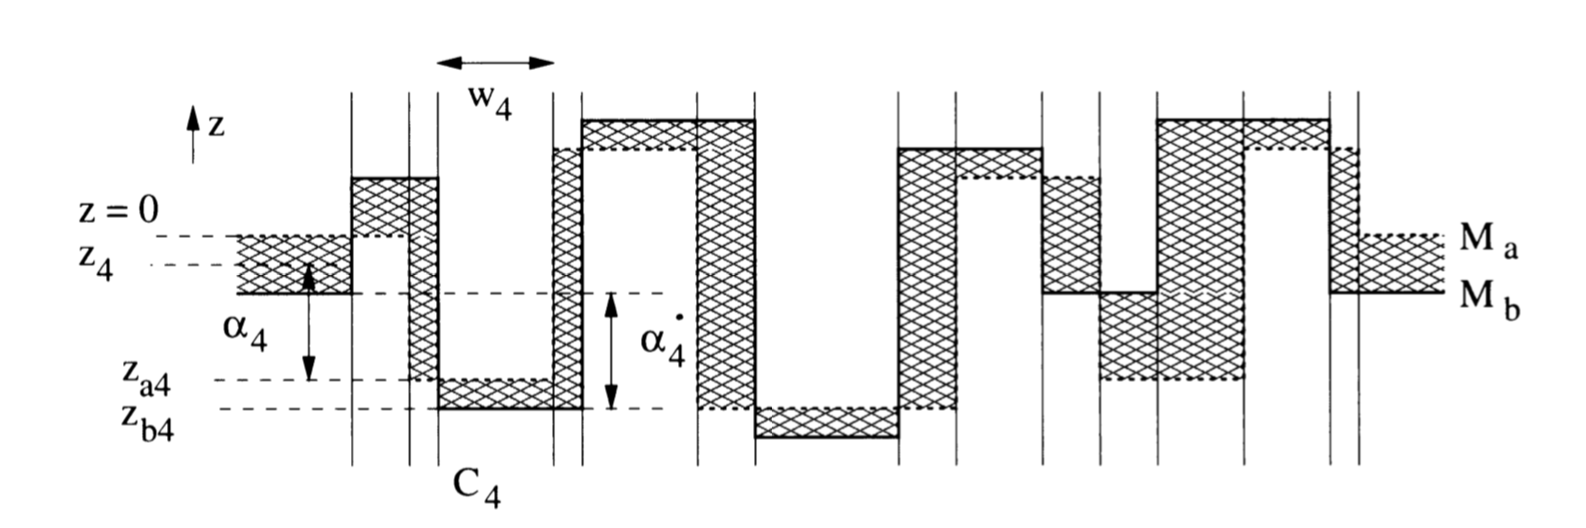
\includegraphics[width=300px,height=100px,keepaspectratio]{abb_2}
		\end{figure}
	\end{frame}
\end{document}